\documentclass[unicode,12pt,aspectratio=169]{beamer}
\usetheme{v2SimpleStyle}
\usepackage{color}
\usepackage{hyperref}
\usepackage{url}
\usepackage{docmute}
\usepackage{graphicx}

% テーマカラー
\definecolor{themeColor}{HTML}{E03200}

% レイアウト関連の設定(お好みで)
\hyphenpenalty=10000
\setlength\abovecaptionskip{0pt}

% フォント設定(メイリオがない環境だと動かないと思う=書き換えて)
\usepackage{zxjatype}
\renewcommand{\bfdefault}{bx}
\setCJKmainfont[Scale=0.95]{Meiryo}
\renewcommand\UrlFont{Meiryo}
\setsansfont[
    BoldFont={Meiryo Bold},
    ItalicFont={Meiryo Italic},
    BoldItalicFont={Meiryo Italic}
]{Fira Sans}

% 日本語化
\renewcommand{\figurename}{図}
\renewcommand{\tablename}{表}

% 情報(画像パスと出力するPDFの設定)
\graphicspath{{images/}}
\hypersetup{
  pdftitle={北海道の回転寿司と100円寿司の違い},
  pdfauthor={TomSuzuki}
}

% タイトル設定(書くことは英語の通り)
\title{北海道の回転寿司と100円寿司の違い}
\subtitle{The Difference Between Conveyor-Belt Sushi and 100 yen Sushi in Hokkaido}
\author{TomSuzuki}
\institute{2021年度 お寿司を語る会}
\date{2021年11月7日}

% 本体
\begin{document}
    \begin{frame}[plain,c]
    \titlepage
\end{frame}

    \begin{frame}[fragile,c]{お寿司とは}
    \centering
    \textbf{寿司} ...一般に米飯などと主に魚介類を組み合わせた和食\cite{sushi_wikipedia}。\\
     \\
    
    \begin{figure}
        \centering
        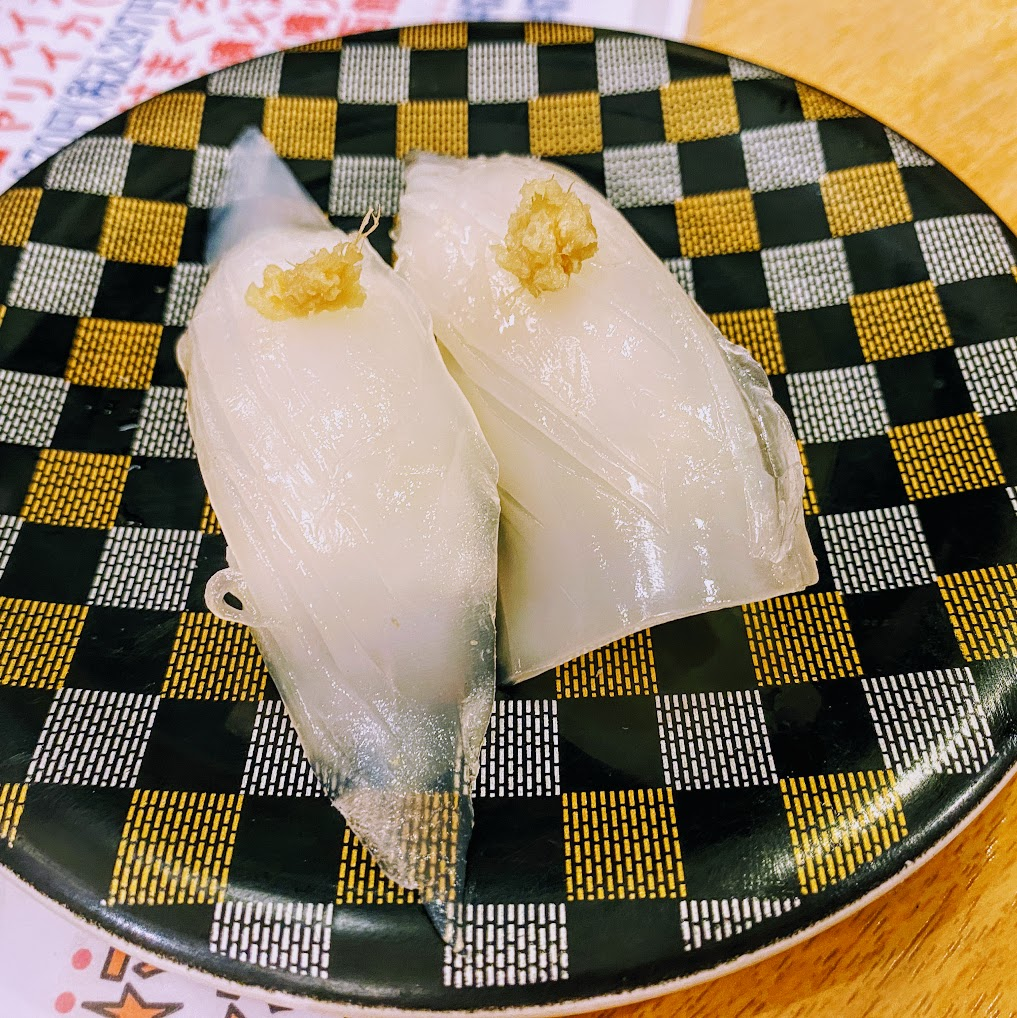
\includegraphics[width=3cm]{ika}
        \caption{函館名物「イカ」}
        \label{fig:ika}
    \end{figure}

    \pagereference[{\cite{sushi_wikipedia} Wikipedia. 寿司. \url{https://ja.wikipedia.org/wiki/\%E5\%AF\%BF\%E5\%8F\%B8} (参照: 2021-11-07)}]
\end{frame}

    \begin{frame}[fragile,c]{100円寿司のサーモン}
    \centering

    \begin{figure}[H]
        \begin{minipage}{0.55\hsize}
            \centering
            ネタが小さい\\
            おなかすいてきた\\
             \\
            お手頃価格(?)\\
        \end{minipage}
        \begin{minipage}{0.4\hsize}
            \centering
            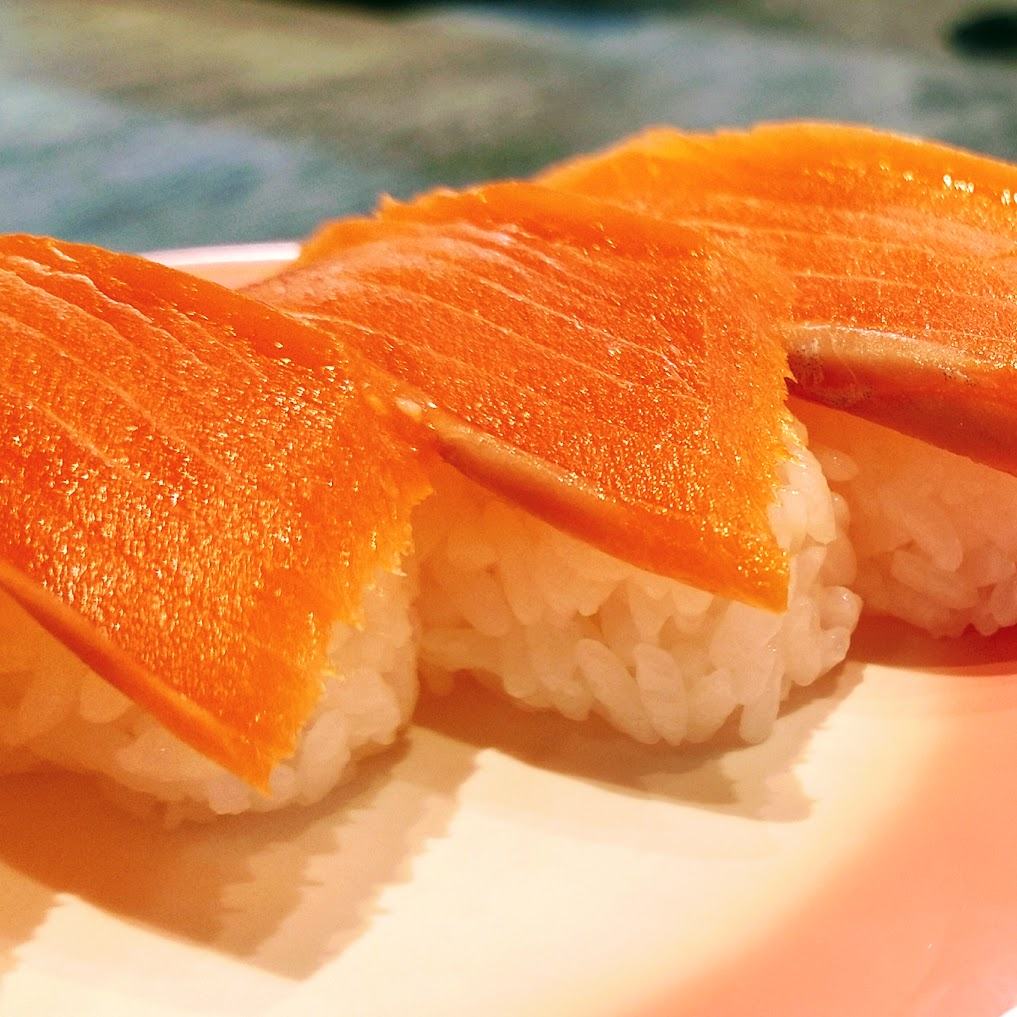
\includegraphics[width=0.95\hsize]{100yen}
            \caption{一般的な100円寿司のサーモン}
            \label{fig:100yen}
        \end{minipage}
    \end{figure}

\end{frame}

    \begin{frame}[fragile,c]{北海道の回転寿司のサーモン}
    \centering

    \begin{figure}[H]
        \begin{minipage}{0.55\hsize}
            \centering
            ネタが\textbf{大きい}\\
            なんか\alert{美味しそう}\\
             \\
            でも高い...\\
        \end{minipage}
        \begin{minipage}{0.4\hsize}
            \centering
            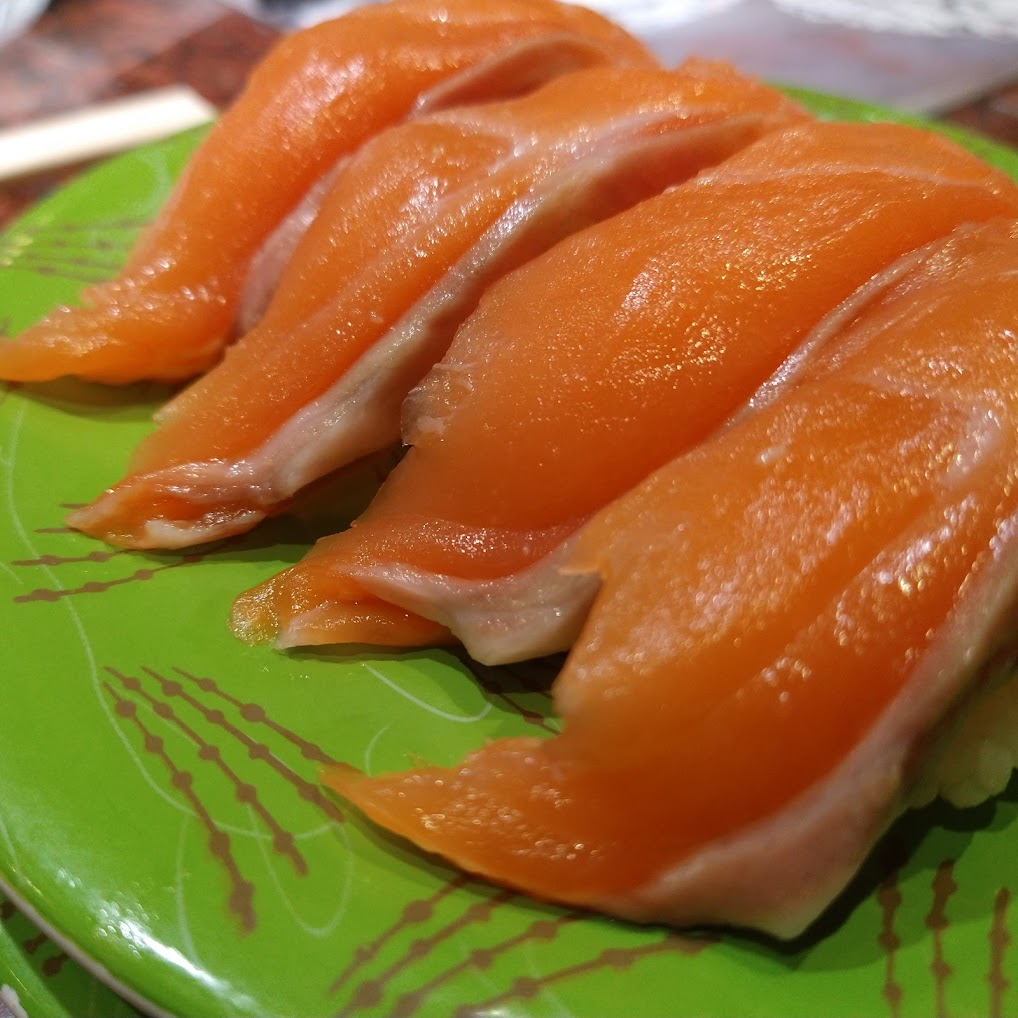
\includegraphics[width=0.95\hsize]{hokkaido}
            \caption{北海道の回転寿司のサーモン}
            \label{fig:hokkaido}
        \end{minipage}
    \end{figure}

\end{frame}

    \begin{frame}[fragile,c]{まとめ}
    \setlength{\leftmargini}{1em}

    \begin{figure}[H]
        \begin{minipage}[b]{0.55\hsize}
            \textbf{ポイント}
            \begin{itemize}
                \item 寿司は\alert{美味しい}
                \item おなかすいた
                \item Wikipediaは参考文献にならない
            \end{itemize}
             \\
            \textbf{今後の課題}
            \begin{itemize}
                \item 他都府県のお寿司はどうなのか
            \end{itemize}
        \end{minipage}
        \begin{minipage}[t]{0.4\hsize}
            \centering
            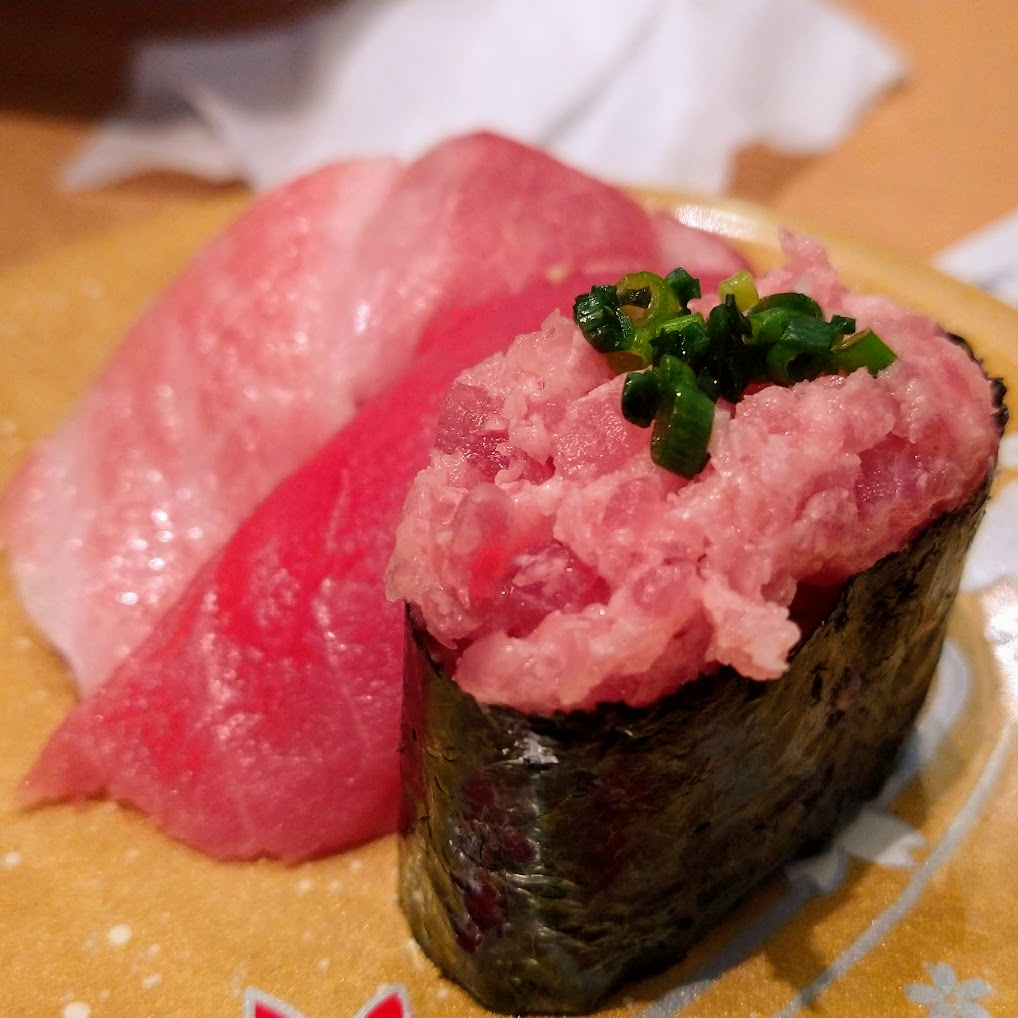
\includegraphics[width=0.95\hsize]{oishii}
            \caption{美味しい寿司}
            \label{fig:oishii}
        \end{minipage}
    \end{figure}

\end{frame}

    \bibliographystyle{junsrt}
\begin{frame}[t]{参考文献}%other option: allowframebreaks
    \scriptsize
    \beamertemplatetextbibitems
    \bibliography{reference}
\end{frame}

\end{document}
